\documentclass[a4paper,11.5pt, table]{article}

%%%%%% Basic packages begin %%%%%%
\usepackage[
	textwidth  = 160mm, 
	textheight = 230mm, 
	top        = 25mm, 
	bottom     = 30mm
]{geometry}
\usepackage[normalem]{ulem}
\usepackage[utf8]{inputenc}
\usepackage[T1]{fontenc}
\PassOptionsToPackage{defaults=hu-min}{magyar.ldf}
\usepackage[magyar]{babel}

%%%%%%% Basic packages end %%%%%%%

%%%%%% Packages required for this document begin %%%%%%
\usepackage{
	amsmath,   % Math mode
	amsthm,    % "note" environment
	amsfonts,  % "\mathbb{}" command
	paralist,  % "compactitem" and "compactenum" environment
	multirow,  % "\multirow{}{}" command
	float,     % "H" float specifier
	tikz,      % Basepackage for nearly all figures
	listings,  % Used for code snippets
	etaremune, % Reverse compactenum
%	graphicx   % For including images
	enumitem   %for alphabetical enumeration
}
\usepackage[unicode]{hyperref} % Clickable links
%%%%%%% Packages required for this document end %%%%%%%

%%%%%% TikZ options start %%%%%%
\usetikzlibrary{
	positioning, % Contains positioning utilities, such as "below = of" 
	calc,        % Adding coordinates
	math         % Needed for global variables
}

\tikzstyle{NodeBase} = [
	rectangle,
	text centered,
	draw = black
]

\definecolor{DefaultObjectColor}{gray}{0.9} % This is the default color of object in the TikZ pictures

\tikzstyle{arrow} = [
	thick,
	->,
	>=stealth
]
%%%%%%% TikZ options end %%%%%%%

%%%%%% lstlistings envvironment options start %%%%%%

\lstdefinestyle{customc}{ % C/C++ code snippet style
	belowcaptionskip = 1\baselineskip,
	breaklines       = true,
	frame            = L, % Double line on the left
	language         = C++,
	showstringspaces = false,
	basicstyle       = \ttfamily,
	keywordstyle     = \bfseries\color{green!40!black},
	stringstyle      = \color{orange},
	emphstyle        = \color{blue}, % Defined below
	tabsize          = 4,
	columns          = fullflexible,
}

\lstset{
	escapechar = @,
	style      = customc, % Default code snippet style
	%NOTE In order to use special characters in code snippets, one has to manually define them.
	literate   = {á}{{\'a}}1 {é}{{\'e}}1 {í}{{\'i}}1 {ó}{{\'o}}1 {ú}{{\'u}}1	{Á}{{\'A}}1 {É}{{\'E}}1 {Í}{{\'I}}1 {Ó}{{\'O}}1 {Ú}{{\'U}}1	{ö}{{\"o}}1 {ü}{{\"u}}1 {Ö}{{\"O}}1 {Ü}{{\"U}}1
	{ű}{{\H{u}}}1 {Ű}{{\H{U}}}1 {ő}{{\H{o}}}1 {Ő}{{\H{O}}}1
	{€}{{\euro}}1 {£}{{\pounds}}1 {~}{$\sim$}{1}	
}

%%%%%%% lstlistings envvironment options end %%%%%%%

%%%%%%%% Compilation error fix begin %%%%%%%%
\makeatletter
\expandafter\let\csname active@char\string?\endcsname\relax
\expandafter\let\csname active@char\string!\endcsname\relax
\expandafter\let\csname active@char\string:\endcsname\relax

\initiate@active@char{?}
\initiate@active@char{!}
\initiate@active@char{:}
\makeatletter
%%%%%%%%% Compilation error fix end %%%%%%%%%

\setlength{\parindent}{0mm}
\setlength{\parskip}{1em}
\setcounter{section}{0}

\begin{document}
	\begin{center}
		{\Huge Adatbázisok II}
		\smallskip
		
		{\Large VI. Ellenőrzőkérdések}
	\end{center}

\section{A konkurenciavezérlés}

189. Milyen problémát kell megoldania a konkurrencia-vezérlésnek? (4 pont)
	\begin{compactitem}
		\item A tranzakciók közötti egymásra hatás az adatbázis-állapot inkonzisztenssé válását okozhatja, még akkor is, amikor a tranzakciók külön-külön megőrzik a konzisztenciát, és rendszerhiba sem történt. 
		\item \textit{MJ.: Akkor fordulhat elő ilyen, ha két, egyszerre futó tranzakció ugyan azt az adatrészt módosítja.}
	\end{compactitem}

190. Mit hívunk ütemezőnek? (2 pont)
	\begin{compactitem}
		\item Az adatbázis-kezelő azon részét hívjuk ütemezőnek (scheduler), amely a tranzakciós lépések szabályozásának feladatát végzi.
	\end{compactitem}

191. Mit hívunk ütemezésnek? (2 pont)
	\begin{compactitem}
		\item Az ütemezés \textit{(schedule)} egy vagy több tranzakció által végrehajtott lényeges műveletek időrendben vett sorozata, amelyben az egy tranzakcióhoz tartozó műveletek sorrendje megegyezik a tranzakcióban megadott sorrenddel. 
	\end{compactitem}

192. Milyen 2 módon biztosítja az ütemező a sorbarendezhetőséget? (2 pont)
	\begin{compactitem}
		\item Várakoztat, abortot rendel el, hogy a sorbarendezhetőséget biztosítsa.
	\end{compactitem}

193. Mit hívunk konfliktuspárnak? (2 pont)
	\begin{compactitem}
		\item A konfliktus \textit{(conflict)} vagy konfliktuspár olyan egymást követő műveletpár az ütemezésben, amelynek ha a sorrendjét felcseréljük, akkor legalább az egyik tranzakció viselkedése megváltozhat.
	\end{compactitem}

194. Milyen 3 esetben nem cserélhetjük fel a műveletek sorrendjét, mert inkonzisztenciát okozhatna? (3 pont)
\begin{compactitem}
	\item Legyen T$_{i}$ és T$_{j}$ két különböző tranzakció (i $\not=$ j).
	\begin{enumerate}[label= \alph*)]
		\item r$_{i}$(X); w$_{i}$(Y) konfliktus,
		\begin{compactitem}
			\item M
			ivel egyetlen tranzakción belül a műveletek sorrendje rögzített, és az adatbázis-kezelő ezt a sorrendet nem rendezheti át.
		\end{compactitem}
		
		\item w$_{i}$(X); w$_{j}$(X) konfliktus, 
		\begin{compactitem}
			\item Mivel mind a kettőt ugyan azt az adatot módosítja. (Ha felcserélnénk őket, más lehet az eredmény.)
		\end{compactitem}
		
		\item r$ _{i} $(X); w$ _{j} $(X) és w$ _{i} $(X); r$ _{j} $(X) is konfliktus. 
		\begin{compactitem}
			\item Ha megcserélnénk a sorrendet, egyrészt az írások miatt más lenne az olvasott adat, másrészt a felcserélt írások sorrendje miatt X értékének a 4 művelet utáni változata is megváltozhat. (És ez a csere azt is jelentené, hogy tranzakción belüli sorrendet cserélünk fel.)
		\end{compactitem}
	\end{enumerate}
\end{compactitem}

195. Mikor konfliktus-ekvivalens 2 ütemezés? (2 pont)
	\begin{compactitem}
		\item Azt mondjuk, hogy két ütemezés konfliktusekvivalens \textit{(conflict-equivalent)}, ha szomszédos műveletek nem konfliktusos cseréinek sorozatával az egyiket átalakíthatjuk a másikká. 
	\end{compactitem}

196. Mikor konfliktus-sorbarendezhető egy ütemezés? (2 pont)
	\begin{compactitem}
		\item Azt mondjuk, hogy egy ütemezés konfliktus-sorbarendezhető \textit{(conflict-serializable schedule)}, ha konfliktusekvivalens valamely soros ütemezéssel. 
		\item \textit{MJ.: Azaz nem konfliktusos cserékkel átvihető az egyik a másikba.}
	\end{compactitem}

197. Mi a konfliktus-sorbarendezhetőség elve? (3 pont)
	\begin{compactitem}
		\item ELV: nem konfliktusos cserékkel az ütemezést megpróbáljuk soros ütemezéssé átalakítani. Ha ezt meg tudjuk tenni, akkor az eredeti ütemezés sorbarendezhető volt, ugyanis az adatbázis állapotára való hatása változatlan marad minden nem konfliktusos cserével.
		\item \textit{Megjegyzés: Két tranzakciónak két soros ütemezése van, az egyikben T$ _{1} $ megelőzi T$ _{2} $‑t, a másikban T$ _{2} $ előzi meg T$ _{1} $-et.}
	\end{compactitem}

198. Mi a kapcsolat a sorbarendezhetőség és a konfliktus-sorbarendezhetőség között? (2 pont)
	\begin{compactitem}
		\item Azt mondjuk, hogy egy ütemezés konfliktus-sorbarendezhető \textit{(conflict-serializable schedule)}, ha konfliktusekvivalens valamely soros ütemezéssel. 
		\begin{compactitem}
			\item Azaz nem konfliktusos cserék által valamely soros ütemezést kaphatjuk.
		\end{compactitem}
		
		\item A konfliktus-sorbarendezhetőség elégséges feltétel a sorbarendezhetőségre, vagyis egy konfliktus-sorbarendezhető ütemezés sorbarendezhető ütemezés is egyben. 
	\end{compactitem}

199. Az r$ _{1} $(A); w$ _{1} $(A); r$ _{2} $(A); w$ _{2} $(A); r$ _{1} $(B); w$ _{1} $(B); r$ _{2} $(B); w$ _{2} $(B); ütemezést alakítsuk soros ütemezéssé (5 pont)
	\begin{compactitem}
		\item Azt állítjuk, hogy ez az ütemezés konfliktus-sorbarendezhető. A következő cserékkel ez az ütemezés átalakítható a (T$ _{1} $, T$ _{2} $) soros ütemezéssé, ahol az összes T$ _{1} $-beli művelet megelőzi az összes T$ _{2} $-beli műveletet:
	\end{compactitem}
\begin{figure}[h]
	\centering
	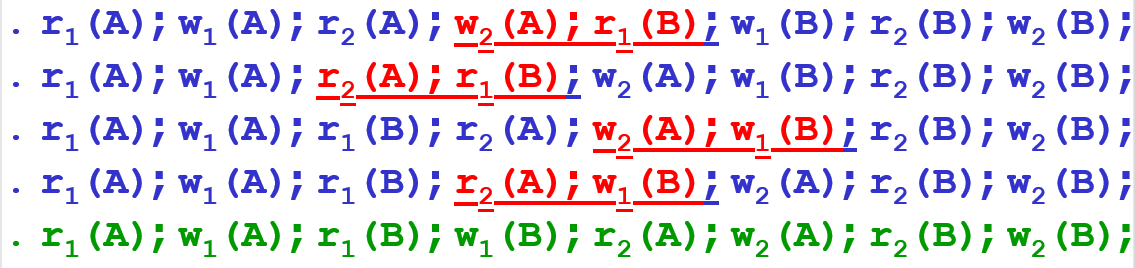
\includegraphics[height=3cm]{01.png}
\end{figure}

200. Adjunk példát sorbarendezhető, de nem konfliktus-sorbarendezhető ütemezésre (4 pont)
	\begin{compactitem}
		\item S$ _{2} $: w$ _{1} $(Y); w$ _{2} $(Y); w$ _{2} $(X); w$ _{1} $(X); w$ _{3} $(X);
	\end{compactitem}

201. Mi a konfliktus-sorbarendezhetőség tesztelésének alapötlete? (2 pont)
	\begin{compactitem}
		\item Alapötlet: ha valahol konfliktusban álló műveletek szerepelnek S-ben, akkor az ezeket a műveleteket végrehajtó tranzakcióknak ugyanabban a sorrendben kell előfordulniuk a konfliktus-ekvivalens soros ütemezésekben, mint ahogyan az S-ben voltak.
	\end{compactitem}

202. Mikor mondjuk, hogy egy S ütemezés alapján T$ _{1} $ megelőzi T$ _{2} $-t? (5 pont)
	\begin{compactitem}
		\item Adott a T$ _{1} $ és T$ _{2} $, esetleg további tranzakcióknak egy S ütemezése. Azt mondjuk, hogy T$ _{1} $ megelőzi T$ _{2} $‑t, ha van a T$ _{1} $-ben olyan A$ _{1} $ művelet és a T$ _{2} $-ben olyan A$ _{2} $ művelet, hogy
		\begin{enumerate}
			\item A$ _{1} $ megelőzi A$ _{2} $-t S-ben,
			\item A$ _{1} $ és A$ _{2} $ ugyanarra az adatbáziselemre vonatkoznak, és
			\item A$ _{1} $ és A$ _{2} $ közül legalább az egyik írás művelet.
		\end{enumerate}
		\item MJ.:
		\begin{compactitem}
			\item Másképpen fogalmazva: A$ _{1} $ és A$ _{2} $ konfliktuspárt alkotna, ha szomszédos műveletek lennének. Jelölése: T$ _{1} $ <$ _{S} $ T$ _{2} $. 
			\item Látható, hogy ezek pontosan azok a feltételek, amikor nem lehet felcserélni A$ _{1} $ és A$ _{2} $ sorrendjét. Tehát A$ _{1} $ az A$ _{2} $ előtt szerepel bármely S-sel konfliktusekvivalens ütemezésben. Ebből az következik, hogy ha ezek közül az ütemezések közül az egyik soros ütemezés, akkor abban T$ _{1} $-nek meg kell előznie T$ _{2} $‑t.
		\end{compactitem}
	\end{compactitem}

203. Adjuk meg egy S ütemezéshez tartozó megelőzési gráf definícióját! (5 pont)
	\begin{compactitem}
		\item Az utóbbi kérdésnél leírt megelőzéseket a megelőzési gráfban \textit{(precedence graph)} összegezhetjük. A megelőzési gráf csúcsai az S ütemezés tranzakciói. Ha a tranzakciókat T$ _{i} $-vel jelöljük, akkor a T$ _{i} $-nek megfelelő csúcsot az i egész jelöli. Az i csúcsból a j csúcsba akkor vezet irányított él, ha T$ _{i} $ <S T$ _{j} $.
	\end{compactitem}

204. Milyen kapcsolat van a konfliktus-ekvivalencia és a megelőzési gráfok között? (4 pont)
	\begin{compactitem}
		\item Lemma: S$ _{1} $, S$ _{2} $ konfliktusekvivalens $ \implies $ gráf(S$ _{1} $) = gráf(S$ _{2} $)
		\item Megjegyzés: gráf(S$ _{1} $) = gráf(S$ _{2} $) $ \not\Rightarrow $ S$ _{1} $, S$ _{2} $ konfliktusekvivalens
	\end{compactitem}

205. Adjunk példát arra, hogy két ütemezés megelőzési gráfja megegyezik, de nem konfliktus-ekvivalensek!(4 pont)
	\begin{compactitem}
		\item Ellenpélda:
		\begin{compactitem}
			\item S$ _{1} $=w$ _{1} $(A) r$ _{2} $(A) w$ _{2} $(B) r$ _{1} $(B)
			\item S$ _{2} $=r$ _{2} $(A) w$ _{1} $(A) r$ _{1} $(B) w$ _{2} $(B)
		\end{compactitem}
			\begin{figure}[h]
				\centering
				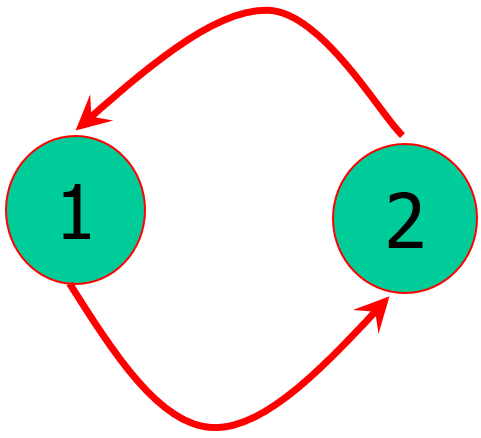
\includegraphics[height=2cm]{02.png}
			\end{figure}
	\end{compactitem}


206. Mit hívunk egy irányított, körmentes gráf esetében a csúcsok topologikus sorrendjének? (4 pont)
	\begin{compactitem}
		\item Egy körmentes gráf csúcsainak topologikus sorrendje a csúcsok bármely olyan rendezése, amelyben minden \textit{a $ \rightarrow $ b} élre az \textit{a} csúcs megelőzi a \textit{b} csúcsot a topologikus rendezésben.
	\end{compactitem}

207. Hogyan lehet tesztelni a megelőzési gráf alapján egy ütemezés konfliktus-sorbarendezhetőségét? (4 pont)
	\begin{compactitem}
		\item Ha az S megelőzési gráf tartalmaz irányított kört, akkor S nem konfliktus-sorbarendezhető, ha nem tartalmaz irányított kört, akkor S konfliktus-sorbarendezhető, és a csúcsok bármelyik topologikus sorrendje megadja a konfliktusekvivalens soros sorrendet.
	\end{compactitem}

208. Mi jellemző a passzív ütemezésre? (4 pont)
	\begin{compactitem}
		\item \textit{MJ.: A passzív ütemezés az ütemező egy eszköze a sorbarendezhetőség elérésére.}
		\item Passzív módszer: 
		\begin{enumerate}
			\item hagyjuk a rendszert működni, 
			\item az ütemezésnek megfelelő gráfot tároljuk, 
			\item egy idő után megnézzük, hogy van-e benne kör, 
			\item és ha nincs, akkor szerencsénk volt, jó volt az ütemezés.
		\end{enumerate}
	\end{compactitem}

209. Mi jellemző az aktív ütemezésre és milyen 3 módszert lehet erre használni? (5 pont)
	\begin{compactitem}
		\item \textit{MJ.: Az aktív ütemezés az ütemező egy eszköze a sorbarendezhetőség elérésére.}
		\item Aktív módszer: az ütemező beavatkozik, és megakadályozza, hogy kör alakuljon ki. 
		\item Az ütemezőnek több lehetősége is van arra, hogy kikényszerítse a sorbarendezhető ütemezéseket:
		\begin{compactitem}
			\item zárak (ezen belül is még: protokoll elemek, pl. 2PL)
			\item időbélyegek (time stamp)
			\item érvényesítés
		\end{compactitem}
		\item \textit{Fő elv: inkább legyen szigorúbb és ne hagyjon lefutni egy olyan ütemezést, ami sorbarendezhető, mint hogy fusson egy olyan, ami nem az.}
	\end{compactitem}

\section{Zárak használata}

210. Mit hívunk a tranzakciók konzisztenciájának zárolási ütemező esetén? (2 pont)
	\begin{compactitem}
		\item \textit{MJ:: A zárolási ütemező a konfliktus-sorbarendezhetőséget követeli meg, (ez erősebb követelmény, mint a sorbarendezhetőség).}
		\item Tranzakciók konzisztenciája (consistency of transactions):
		\begin{compactitem}
			\item A tranzakció csak akkor olvashat vagy írhat egy elemet, ha már korábban zárolta azt, és még nem oldotta fel a zárat.
			\item Ha egy tranzakció zárol egy elemet, akkor később azt fel kell szabadítania.
		\end{compactitem}
	\end{compactitem}
	
211. Mit hívunk a zárolási ütemező jogszerűségének? (1 pont)
	\begin{compactitem}
		\item Az ütemezések jogszerűsége\textit{ (legality of schedules)}: 
		Nem zárolhatja két tranzakció ugyanazt az elemet, csak úgy, ha az egyik előbb már feloldotta a zárat.
	\end{compactitem}

212. Adjunk példát konzisztens tranzakciók jogszerű ütemezésére, ami mégsem sorbarendezhető! (6 pont)
	\begin{compactitem}
		\item Ez az ütemezés jogszerű, de nem sorba rendezhető. 
		\begin{figure}[h]
			\centering
			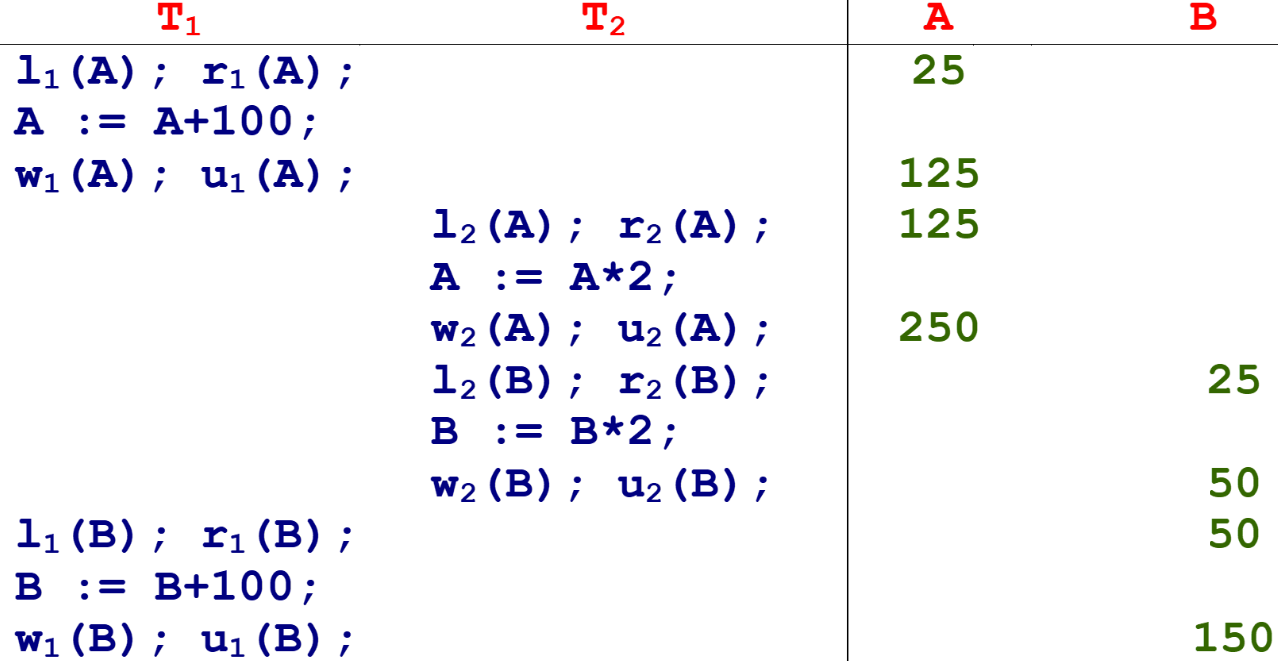
\includegraphics[height=6cm]{03.png}
		\end{figure}
		
		\item Megjegyzés:
		\begin{compactitem}
			\item Kibővítjük a jelöléseinket a zárolás és a feloldás műveletekkel:
			\begin{compactitem}
				\item l$ _{i} $(X): a T$ _{i} $ tranzakció az X adatbáziselemre zárolást kér (lock).
				\item u$ _{i} $(X): a T$ _{i} $ tranzakció az X adatbáziselem zárolását feloldja (unlock).
			\end{compactitem}
			\item Konzisztencia: Ha egy T$ _{i} $ tranzakcióban van egy r$ _{i} $(X) vagy egy w$ _{i} $(X) művelet, akkor van korábban egy l$ _{i} $(X) művelet, és van később egy u$ _{i} $(X) művelet, de a zárolás és az írás/olvasás között nincs u$ _{i} $(X).\\
			T$ _{i} $:  … l$ _{i} $(X) … r/w$ _{i} $(X) … u$ _{i} $(X) ...
			 \item Példa konzisztens tranzakciókra:
			 \begin{figure}[h]
			 	\centering
			 	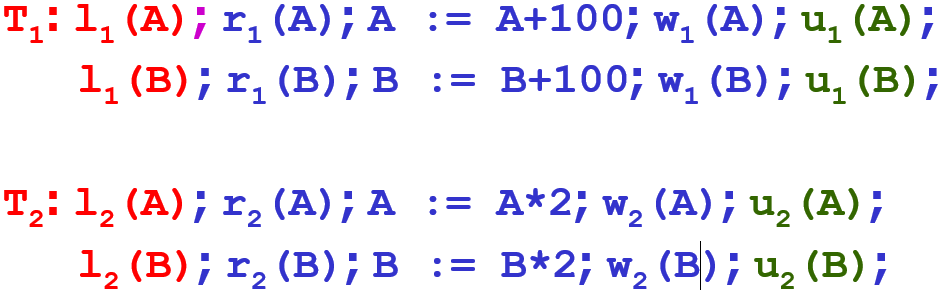
\includegraphics[height=3cm]{04.png}
			 \end{figure}			 
		\end{compactitem}
	\end{compactitem}

213. Mit hívunk kétfázisú zárolásnak és szemléltessük rajzban is? (2 pont)
	\begin{compactitem}
		\item A kétfázisú zárolás\textit{ (two-phase locking, 2PL)}:
		\begin{compactitem}
			\item Szemléletesen:
			\begin{figure}[h]
				\centering
				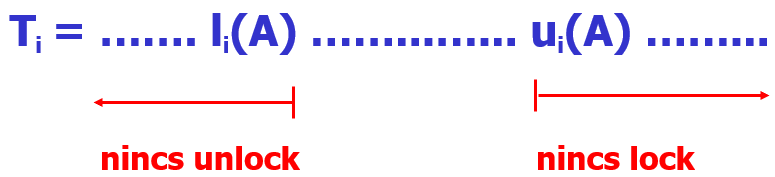
\includegraphics[height=2cm]{05.png}
			\end{figure}
		\item Példa:
			\begin{figure}[h]
				\centering
				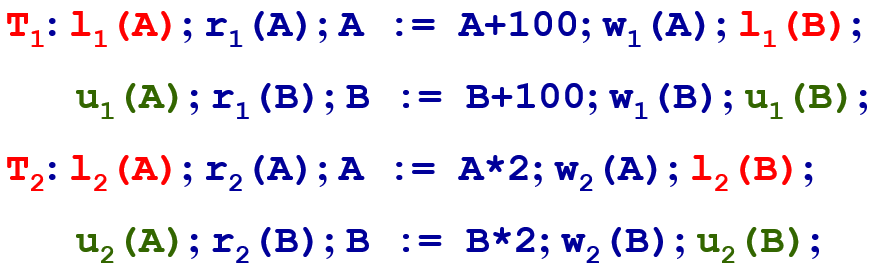
\includegraphics[height=3cm]{06.png}
			\end{figure}
			\item Minden \underline{tranzakcióban} minden zárolási művelet megelőzi az összes zárfeloldási műveletet. (Amíg a műveletei az adott adatot változtatják, addig nem engedi el azt.)
		\end{compactitem}
	\end{compactitem}

214. Adjunk a tranzakciókra 2, az ütemezésre 1 feltételt, ami elegendő a konfliktus-sorbarendezhetőség bizonyítására! Milyen módon bizonyítható a tétel? (5 pont)
	\begin{compactitem}
		\item Tétel: Konzisztens, kétfázisú zárolású tranzakciók bármely S jogszerű ütemezését át lehet alakítani konfliktusekvivalens soros ütemezéssé. 
		\item Bizonyítás: S-ben részt vevő tranzakciók száma (n) szerinti indukcióval. 		
	\end{compactitem}
	
\subsection{A holtpont}
	
215. Mi a várakozási gráf és hogyan segít a holtpont felismerésében? (4 pont)
	\begin{compactitem}
		\item \textit{A holtpont: amikor egyik tranzakció sem folytatódhat, hanem örökké várakozniuk kell.} 
		\begin{figure}[h]
			\centering
			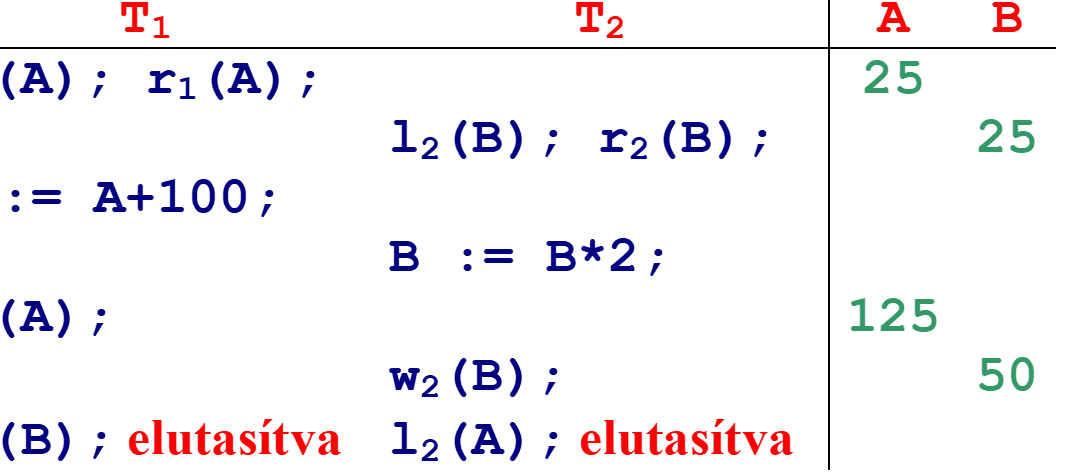
\includegraphics[height=4cm]{07.png}
		\end{figure}
		\item Várakozási gráf: csúcsai a tranzakciók és akkor van él T$ _{i} $-ből T$ _{j} $-be, ha T$ _{i} $ vár egy olyan zár elengedésére, amit Tj tart éppen.
		\item Tétel: Az ütemezés során egy adott pillanatban pontosan akkor nincs holtpont, ha az adott pillanathoz tartozó várakozási gráfban nincs irányított kör.		
	\end{compactitem}
		
216. Milyen két lehetőséggel védekezhetünk a holtpont ellen? (4 pont)
	\begin{enumerate}[label = \alph*)]
		\item Minden egyes tranzakció előre elkéri az összes zárat, ami neki kelleni fog. Ha nem kapja meg az összeset, akkor egyet se kér el, el se indul.
		Ilyenkor biztos nem lesz holtpont, mert ha valaki megkap egy zárat, akkor le is tud futni, nem akad el. Az csak a baj ezzel, hogy előre kell mindent tudni.
		\item Feltesszük, hogy van egy sorrend az adategységeken és minden egyes tranzakció csak eszerint a sorrend szerint növekvően kérhet újabb zárakat. Itt lehet, hogy lesz várakozás, de holtpont biztos nem lesz. Miért?
	\end{enumerate}

217. Mi a kiéheztetés problémája és milyen megoldás van rá? (2 pont)
	\begin{compactitem}
		\item Kiéhezés: többen várnak ugyanarra a
		zárra, de amikor felszabadul mindig elviszi valaki a tranzakció orra elől.
		\item Megoldás: adategységenként FIFO listában tartani a várakozókat, azaz mindig a legrégebben várakozónak adjuk oda a zárolási lehetőséget.		
	\end{compactitem}

\subsection{Oszott és kizárólagos zárak}

Bevezetés:
	\begin{compactitem}
		\item A legelterjedtebb zárolási séma két különböző zárat alkalmaz: az osztott zárakat\textit{ (shared locks)} vagy olvasási zárakat, és a kizárólagos zárakat\textit{ (exclusive locks)} vagy írási zárakat. 
		\item Tetszőleges X adatbáziselemet vagy egyszer lehet zárolni kizárólagosan, vagy akárhányszor lehet zárolni osztottan, ha még nincs kizárólagosan zárolva. 
		\item Amikor írni akarjuk X-et, akkor X-en kizárólagos zárral kell rendelkeznünk, de ha csak olvasni akarjuk, akkor X-en akár osztott, akár kizárólagos zár megfelel. 
		\item Feltételezzük, hogy ha olvasni akarjuk X-et, de írni nem, akkor előnyben részesítjük az osztott zárolást.
		\item Jelölések:
		\begin{compactitem}
			\item sl$ _{i} $(X): T$ _{i} $ tranzakció osztott zárat kér az X adatbáziselemre.
			\item xl$ _{i} $(X): T$ _{i} $ kizárólagos zárat kér X-re.
			\item u$ _{i} $(X): T$ _{i} $ felszabadítja X-et minden zár alól.
		\end{compactitem}
	\end{compactitem}

218. Osztott és kizárólagos zárak esetén mit hívunk a tranzakció konzisztenciájának? (2 pont)
	\begin{compactitem}
		\item Nem írhatunk kizárólagos zár fenntartása nélkül, és nem olvashatunk valamilyen zár fenntartása nélkül. 
		\item Minden zárolást követnie kell egy ugyanannak az elemnek a zárolását feloldó műveletnek.
	\end{compactitem}

219. Osztott és kizárólagos zárak esetén mit hívunk az ütemezés jogszerűségének? (2 pont)
	\begin{compactitem}
		\item Az ütemezések jogszerűsége: Egy elemet vagy egyetlen tranzakció zárol kizárólagosan, vagy több is zárolhatja osztottan, de a kettő egyszerre nem lehet. 
	\end{compactitem}

220. Osztott és kizárólagos zárak esetén adjunk meg feltételeket az ütemezés konfliktus-sorbarendezhetőségére? (4 pont)
	\begin{compactitem}
		\item Konzisztens 2PL (2 fázisú) tranzakciók jogszerű ütemezése konfliktus-sorbarendezhető.
	\end{compactitem}

\subsection{Kompatibilitási mátrixok}

221. Osztott és kizárólagos zárak esetén adjuk meg a kompatibilitási mátrixot!(4 pont)
	\begin{compactitem}
		\item Megjegyzés:
		\begin{compactitem}
			\item A kompatibilitási mátrix minden egyes zármódhoz rendelkezik egy-egy sorral és egy-egy oszloppal. 
			\item A sorok egy másik tranzakció által az X elemre elhelyezett záraknak, az oszlopok pedig az X-re kért zármódoknak felelnek meg. 
			\item A kompatibilitási mátrix használatának szabálya:
			Egy A adatbáziselemre C módú zárat akkor és csak akkor engedélyezhetünk, ha a táblázat minden olyan R sorára, amelyre más tranzakció már zárolta A-t R módban, a C oszlopban „igen” szerepel.
		\end{compactitem}
		\item Az osztott (S) és kizárólagos (X) zárak kompatibilitási mátrixa:
		\begin{figure}[h]
			\centering
			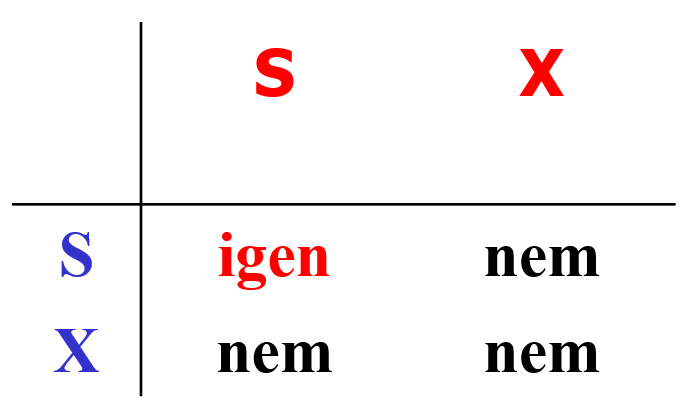
\includegraphics[height=2cm]{08.png}
		\end{figure}
	\end{compactitem}

\newpage
222. Többmódú zárak kompatibilitási mátrixa segítségével hogyan definiáljuk a megelőzési gráfot? (5 pont)
	\begin{compactitem}
		\item A megelőzési gráf csúcsai a tranzakciók és akkor van él T$ _{i} $-ből T$ _{j} $-be, ha van olyan A adategység, amelyre az ütemezés során Z$ _{k} $ zárat kért és kapott T$ _{i} $ ezt elengedte, majd
		\item Ezután A-ra legközelebb T$ _{j} $ kért és kapott olyan Z$ _{l} $ zárat, hogy a mátrixban a Z$ _{k} $ sor Z$ _{l} $ oszlopában \textit{Nem} áll.
	\end{compactitem}
			
223. Többmódú zárak esetén a megelőzési gráf segítségével hogy lehet eldönteni a sorbarendezhetőséget? (3 pont)
	\begin{compactitem}
		\item Tétel: Egy csak zárkéréseket és zárelengedéseket tartalmazó jogszerű ütemezés sorbarendezhető akkor és csak akkor, ha a kompatibilitási mátrix alapján felrajzolt megelőzési gráf nem tartalmaz irányított kört.
	\end{compactitem}

224. Adjunk példát arra, hogy egy zárolási ütemező elutasít sorbarendezhető ütemezést? (4 pont)
	\begin{compactitem}
		\item Tekintsük a következő ütemezést:
		\begin{figure}[h]
			\centering
			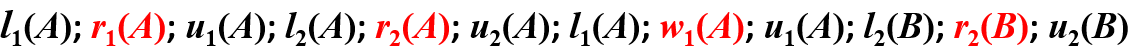
\includegraphics[height=0.5cm]{09.png}
		\end{figure}
		\item Ha megnézzük az írás/olvasás műveleteket (r$ _{1} $(A); r$ _{2} $(A); w$ _{1} $(A); r$ _{2} $(B)), akkor látszik, hogy az ütemezés hatása azonos a T$ _{2} $T$ _{1} $ soros ütemezés hatásával, vagyis ez egy sorbarendezhető ütemezés zárak nélkül.
		\item De ha felrajzoljuk a zárakra vonatkozó megelőzési gráfot (és ilyenkor persze nem nézzük, hogy milyen írások/olvasások vannak, hanem a legrosszabb esetre készülünk), akkor az irányított kört tartalmaz, akkor ezt elvetnénk, mert nem lesz sorbarendezhető az az ütemezés, amiben már
		csak a zárak vannak benne.
		\begin{figure}[h]
			\centering
			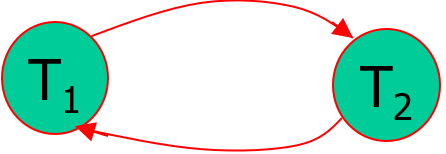
\includegraphics[height=2cm]{10.png}
		\end{figure}
	\end{compactitem}

225. Adjunk feltételt az ütemezés sorbarendezhetőségére tetszőleges zármodellben! (4 pont)
	\begin{compactitem}
		\item Tétel: Ha valamilyen zármodellben egy jogszerű ütemezésben minden tranzakció követi a 2PL-t, akkor az ütemezéshez tartozó megelőzési gráf nem tartalmaz irányított kört, azaz az ütemezés sorbarendezhető.
	\end{compactitem}

226. Mikor mondjuk, hogy egyik zár erősebb a másiknál? (4 pont)
	\begin{compactitem}
		\item L$ _{2} $ erősebb L$ _{1} $ zárnál, ha a kompatibilitási mátrixban L$ _{2} $ sorában /oszlopában minden olyan pozícióban „NEM” áll, amelyben L$ _{1} $ sorában /oszlopában „NEM” áll. 
	\end{compactitem}

227. Adjuk meg a módosítási zár kompatibilitási mátrixát és értelmezzük röviden!(4 pont)
	\begin{compactitem}
		\item\textit{ Megjegyzés: Módosítási zár}
		\begin{compactitem}
			\item Az ul$ _{i} $(X) módosítási zár a T$ _{i} $ tranzakciónak csak X olvasására ad jogot, X írására nem. Később azonban csak a módosítási zárat lehet felminősíteni írásira, az olvasási zárat nem (azt csak módosításira). 
			\item A módosítási zár tehát nem csak a holtpontproblémát oldja meg, hanem a kiéheztetés problémáját is.			
		\end{compactitem}
		\item Az U módosítási zár úgy néz ki, mintha osztott zár lenne, amikor kérjük, és úgy néz ki, mintha kizárólagos zár lenne, amikor már megvan: 
		\begin{figure}[h]
			\centering
			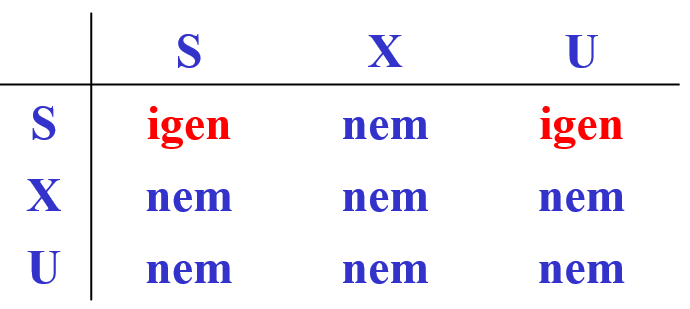
\includegraphics[height=3cm]{11.png}
		\end{figure}
	\end{compactitem}

228. Mi az inc$ _{i} $(X)művelet és adjuk meg a növelési zár kompatibilitási mátrixát! (4 pont)
	\begin{compactitem}
		\item Az inc$ _{i} $(X) művelet:
		\begin{compactitem}
			\item A Ti tranzakció megnöveli az X adatbáziselemet valamely konstanssal. 
			\item (Annak, hogy pontosan mennyi ez a konstans, nincs jelentősége.)
		\end{compactitem}
		\item MJ.: A műveletnek megfelelő növelési zárat \textit{(increment lock)} il$ _{i} $(X)-szel jelöljük.
		\item Növelési zárak:
		\begin{figure}[h]
			\centering
			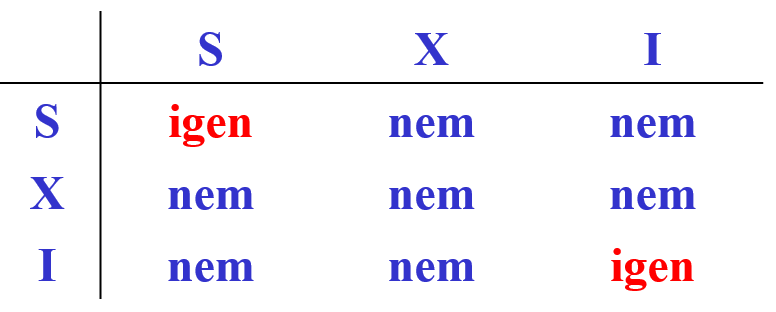
\includegraphics[height=3cm]{12.png}
		\end{figure}
	\end{compactitem}

229. Adjunk meg a zártábla egy lehetséges formáját, a mezők tartalmát magyarázzuk is el! (8 pont)

230. A zárfeloldások sorrendje milyen elvek alapján történhet? (3 pont)
	\begin{compactitem}
		\item Több különböző megközelítés lehetséges, mindegyiknek megvan a saját előnye:
		\begin{enumerate}
			\item Első beérkezett első kiszolgálása \textit{(first-come-first-served)}: \\
			Azt a zárolási kérést engedélyezzük, amelyik a legrégebb óta várakozik. Ez a stratégia azt biztosítja, hogy ne legyen kiéheztetés, vagyis a tranzakció ne várjon örökké egy zárra.
			\item Elsőbbségadás az osztott záraknak \textit{(priority to shared locks)}:\\
			 Először az összes várakozó osztott zárat engedélyezzük. Ezután egy módosítási zárolást engedélyezünk, ha várakozik ilyen. A kizárólagos zárolást csak akkor engedélyezzük, ha semmilyen más igény nem várakozik. Ez a stratégia csak akkor engedi a kiéheztetést, ha a tranzakció U vagy X zárolásra vár.
			\item Elsőbbségadás a felminősítésnek \textit{(priority to upgrading)}:\\
			 Ha van olyan U zárral rendelkező tranzakció, amely X zárrá való felminősítésre vár, akkor ezt engedélyezzük előbb. Máskülönben a fent említett stratégiák valamelyikét követjük.
		\end{enumerate}
	\end{compactitem}
		
231. Hierarchikus adatok esetén mi a figyelmeztető zárak használatának három alapelve? (3 pont)
	\begin{compactitem}
		\item \textit{Megjegyzés: A figyelmeztető protokoll  zárjai (warning protocol):}
		\begin{compactitem}
			\item A közönséges zárak: S és X (osztott és kizárólagos), 
			\item Figyelmeztető zárak: IS, IX (I=intention)\\
			Például IS azt jelenti, hogy szándékunkban áll osztott zárat kapni egy részelemen. 
		\end{compactitem}
		\item A kért zárnak megfelelő figyelmeztető zárakat kérünk az útvonal mentén a gyökérből kiindulva az adatelemig. 
		\item Addig nem megyünk lejjebb, amíg a figyelmeztető zárat meg nem kapjuk.
		\item Így a konfliktusos helyzetek alsóbb szintekre kerülnek a fában.		
	\end{compactitem}

232. Hierarchikus adatok esetén adjuk meg az osztott, kizárólagos és figyelmeztető zárakra vonatkozó kompatibilitási mátrixot? (4 pont)
	\begin{compactitem}
		\begin{figure}[h]
			\centering
			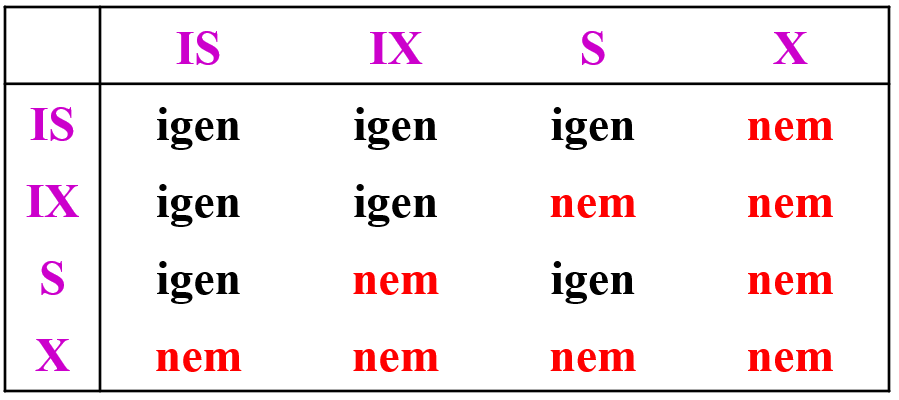
\includegraphics[height=4cm]{13.png}
		\end{figure}
		\item Oszlop: Megkaphatjuk-e ezt a típusú zárat?
		\item Sor: Ha ilyen zár van már kiadva.
	\end{compactitem}
		
233. Hierarchikus adatok esetén miért vezetjük be az SIX zártípust és mi jellemző rá? (4 pont)
	\begin{compactitem}
		\item IS<IX és S<X, de IX és S nem összehasonlítható (< csak parciális rendezés).
		\item A csoportos mód használatához vezessünk be egy SIX új zárat, (ami azt jelenti, hogy ugyanaz a tranzakció S és IX zárat is tett egy adatelemre). Ekkor SIX mindkettőnél erősebb, de ez a legkisebb ilyen.
	\end{compactitem}		
 
234. Adjuk meg a csoportos móddal kiegészített figyelmeztető zárakra vonatkozó kompatibilitási mátrixot! (5 pont)
	\begin{compactitem}
		\begin{figure}[h]
			\centering
			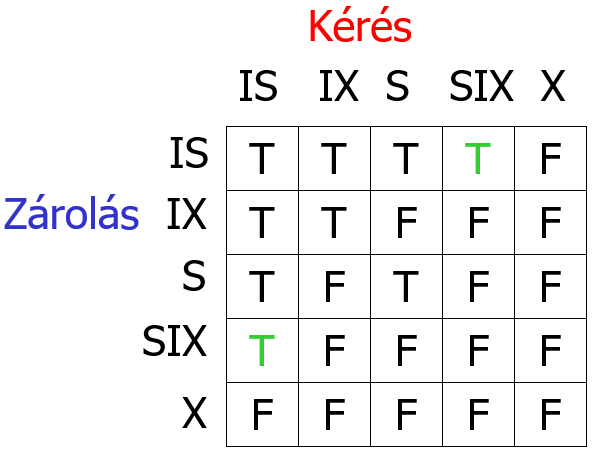
\includegraphics[height=4cm]{14.png}
		\end{figure}
		\item T \textit{(true)} = igen.
		\item F \textit{(false)} = nem.
	\end{compactitem}

\subsection{Nem ismételhető olvasás és a fantomok}

235. Mit hívunk nem ismételhető olvasásnak és mi a probléma vele? (4 pont)
	\begin{compactitem}
		\item Tegyük fel, hogy van egy T$ _{1} $ tranzakció, amely egy adott feltételnek eleget tevő sorokat válogat ki egy relációból. Ezután hosszas számításba kezd, majd később újra végrehajtja a fenti lekérdezést. 
		\item Tegyük fel továbbá, hogy a lekérdezés két végrehajtása között egy T$ _{2} $ tranzakció módosít vagy töröl a táblából néhány olyan sort, amely eleget tesz a lekérdezés feltételének. 
		\item A T$ _{1} $ tranzakció lekérdezését ilyenkor nem ismételhető (fuzzy) olvasásnak nevezzük. 
		\item A nem ismételhető olvasással az a probléma, hogy mást eredményez a lekérdezés másodszori végrehajtása, mint az első. 
		\item\textit{ Megjegyzés:} A tranzakció viszont elvárhatja (ha akarja), hogy ha többször végrehajtja ugyanazt a lekérdezést, akkor mindig ugyanazt az eredményt kapja.
	\end{compactitem}

236. Mit hívunk fantom soroknak? (3 pont)
	\begin{compactitem}
		\item Ugyanez a helyzet akkor is, ha a T$ _{2} $ tranzakció beszúr olyan sorokat, amelyek eleget tesznek a lekérdezés feltételének. A lekérdezés másodszori futtatásakor most is más eredményt kapunk, mint az első alkalommal. 
		Ennek az az oka, hogy most olyan sorokat is figyelembe kellett venni, amelyek az első futtatáskor még nem is léteztek. 
		Az ilyen sorokat nevezzük fantomoknak (phantom).
	\end{compactitem}
237. Mikor követi egy tranzakció a faprotokollt? Adjuk meg a faprotokoll 4 szabályát! (4 pont)
	\begin{compactitem}
		\item A Ti tranzakció követi a faprotokollt, ha
		\begin{enumerate}
			\item Az első zárat bárhova elhelyezheti.
			\item A későbbiekben azonban csak akkor kaphat zárat A-n, ha ekkor zárja van A apján.
			\item Zárat bármikor fel lehet oldani (nem 2PL).
			\item Nem lehet újrazárolni, azaz ha Ti elengedte egy A adategység zárját, akkor később nem kérhet rá újra (még akkor sem, ha A apján még megvan a zárja).
		\end{enumerate}
	\end{compactitem}		

238. Hierarchiák, például B*-fa elemeinek zárolása esetén milyen feltétel adható az ütemezés sorbarendezhetőségére? (4 pont)
	\begin{compactitem}
		\item Tétel: Ha minden tranzakció követi a faprotokollt egy jogszerű ütemezésben, akkor az ütemezés sorbarendezhető lesz, noha nem feltétlenül lesz 2PL.
	\end{compactitem}

\section{Konkurenciavezérlés időbélyegzőkkel}

Bevezetés:
	\begin{compactitem}
		\item Eddig a zárakkal kényszerítettük ki a sorbarendezhető ütemezést.
		\item Itt két másik módszerről lesz szó a tranzakciók sorbarendezhetőségének biztosítására: időbélyegzés és érvényesítés.
	\end{compactitem}		

239. Mi az időbélyegzési módszer lényege? Használunk-e ilyenkor zárakat? (4 pont)
	\begin{compactitem}
		\item Minden tranzakcióhoz hozzárendelünk egy „időbélyegzőt”. 
		\item Minden adatbáziselem utolsó olvasását és írását végző tranzakció időbélyegzőjét rögzítjük, és összehasonlítjuk ezeket az értékeket, hogy biztosítsuk, hogy a tranzakciók időbélyegzőinek megfelelő soros ütemezés ekvivalens legyen a tranzakciók aktuális ütemezésével.
		\item Ehhez nem használunk zárakat.
	\end{compactitem}		

240. Adjunk meg három jellemzőt az Oracle konkurenciavezérlésére vonatkozóan! (3 pont)
	\begin{compactitem}
		\item Az Oracle alkalmazza a kétfázisú zárolást, a figyelmeztető protokollt és a többváltozatú időbélyegzőket is némi módosítással.
	\end{compactitem}

241. Milyen olvasási konzisztenciát biztosít az Oracle és mivel éri ezt el? (3 pont)
	\begin{compactitem}
		\item Többszintű konkurenciavezérlés Oracle-ben
		\begin{itemize}
			\item Utasítás szintű olvasási konzisztencia:
			\begin{compactitem}
				\item Az Oracle minden lekérdezés számára biztosítja az olvasási konzisztenciát, azaz a lekérdezés által olvasott adatok egy időpillanatból (a lekérdezés kezdetének pillanatából) származnak. 
				\item Emiatt a lekérdezés sohasem olvas piszkos adatot, és nem látja azokat a változtatásokat sem, amelyeket a lekérdezés végrehajtása alatt véglegesített tranzakciók eszközöltek. 
			\end{compactitem}
			
			\item Tranzakció szintű olvasási konzisztencia: Kérhetjük egy tranzakció összes lekérdezése számára is a konzisztencia biztosítását. 
			\begin{compactitem}
				\item Ezt úgy érhetjük el, hogy a tranzakciót sorba rendezhető 
				\item vagy csak olvasás módban futtatjuk. 
				\item Ekkor a tranzakció által tartalmazott összes lekérdezés a tranzakció indításakor fennálló adatbázis-állapotot látja, kivéve a tranzakció által korábban végrehajtott módosításokat.
			\end{compactitem}
		
			\item A kétféle olvasási konzisztencia eléréséhez az Oracle a rollback szegmensekben található információkat használja fel. 		
		\end{itemize}
	\end{compactitem}

242. Adjuk meg az SQL92 ANSI/ISO szabványbanszereplő tranzakciós elkülönítési szinteket! (4 pont)
	\begin{compactitem}
		\item Nem olvasásbiztos.
		\item Olvasásbiztos.
		\item Megismételhető olvasás.
		\item Sorba-rendezhető.
	\end{compactitem}

243. Mi jellemező a nem olvasásbiztos elkülönítési szintre a piszkos, fantom, nem ismételhető olvasásokra vonatkozóan? (3 pont)
	\begin{compactitem}
		\item Piszkos olvasás: lehetséges.
		\item Nem ismételhető olvasás: lehetséges.
		\item Fantomok olvasása: lehetséges.
	\end{compactitem}

244. Mi jellemző az olvasásbiztos elkülönítési szintre a piszkos, fantom, nem ismételhető olvasásokra vonatkozóan? (3 pont)
	\begin{compactitem}
		\item Piszkos olvasás: nem lehetséges.
		\item Nem ismételhető olvasás: lehetséges.
		\item Fantomok olvasása: lehetséges.
	\end{compactitem}

245. Mi jellemző a megismételhető olvasás elkülönítési szintre a piszkos, fantom, nem ismételhető olvasásokra vonatkozóan? (3 pont)
	\begin{compactitem}
	\item Piszkos olvasás: nem lehetséges.
	\item Nem ismételhető olvasás: nem lehetséges.
	\item Fantomok olvasása: lehetséges.
\end{compactitem}

246. Mi jellemző a sorbarendezhető elkülönítési szintre a piszkos, fantom, nem ismételhető olvasásokra vonatkozóan? (3 pont)
	\begin{compactitem}
	\item Piszkos olvasás: nem lehetséges.
	\item Nem ismételhető olvasás: nem lehetséges.
	\item Fantomok olvasása: nem lehetséges.
\end{compactitem}

247. Milyen DML szintű zárakat használ az Oracle? (2 pont)
	\begin{compactitem}
		\item \textit{Megjegyzés:} DML-zárak (adatzárak): az adatok védelmére szolgálnak.
		\item DML-zárakat két szinten kaphatnak a tranzakciók: 
		\begin{compactitem}
			\item sorok szintjén 
			\item és teljes táblák szintjén. 
		\end{compactitem}
	\end{compactitem}

248. Milyen zártípusokat használ az Oracle sorokra és táblákra? (6 pont)
	\begin{compactitem}
		\item Sorok szintjén csak egyféle zármód létezik, a kizárólagos (írási – X). 
		\item Táblák szintjén ötféle zármódot különböztetünk meg: 
		\begin{enumerate}
			\item row share (RS) vagy subshare (SS), 
			\item row exclusive (RX) vagy subexclusive (SX), 
			\item share (S), 
			\item share row exclusive (SRX) vagy share-subexclusive (SSX) 
			\item és exclusive (X).
		\end{enumerate}
	\end{compactitem}

\end{document}